\documentclass[a4paper]{article}

\usepackage[english]{babel}
\usepackage[utf8]{inputenc}
\usepackage{amsmath}
\usepackage{graphicx}
\usepackage[colorinlistoftodos]{todonotes}

\title{Yelp data mining final project report}

\author{Jiaoyang Ma, Wenqi Zheng, Yuxuan Xing, Yibo Yu}


\date{\today}

\begin{document}
\maketitle

\section{Introduction}
\label{sec:introduction}

Online reviews are no jokes today. So long as there are always endless options of entertainment and services, people need advices and recommendations from others. Meanwhile, business reviews and social posts online have changed the way of shaping a company's reputation. Top review websites and platforms, including Google My Business, Facebook, Amazon, Yelp and Trip Advisor have hundreds of millions of average monthly traffic in U.S. alone. If these data truly impacts, what could we do with them?
We will look into restaurants reviews in our project. Through multiple data mining techniques, we wish to answer these questions to a certain extend with our analysis: In a city, is the ratings of a restaurant related to its location, price or cuisine? If a customer wants to find a restaurants with a certain cuisine in a given budget, can we find a neighborhoods in that city which have a better chance for the customer to find a restaurants with high ratings? On the other hand, can a restaurant owner find what are the most-mentioned keywords in reviews as feedbacks to improve their services?

 
\section{The data source}
\label{sec:introduction}

Yelp.com had a monthly average of 29 million unique visitors who visited Yelp via the Yelp app and 64 million unique visitors who visited Yelp via mobile web and more than 148 million reviews written by the end of 2017. [1] 
The Yelp Fusion API allows users to get the local content and user reviews in Yelp.com. 
In this report, we will pick Boston as a sample city for the reason below: The query limit of Yelp Fusion API is 1000. Therefore we must pick a city of middle size that when we fix the cuisine category and the price range, the result we have will be as close to 1000 but not exceeds it, or as we could not know the way of choosing result in the API, there might be some problem caused by not equally choosing the results.


\section{The data mining analysis}
\label{sec:theory}

\subsection{Geographical based clustering}
To find answers to our first question that which area in Boston will have restaurants with higher rating, we will used K-Means and GMM to do the clustering and compare the results. To run the algorithm, we have to first manage our data. We filter out the restaurants that have the rating count less than 20. All restaurants that satisfy the condition are mapped out in the figure below.


\begin{figure}[htbp]
\centering
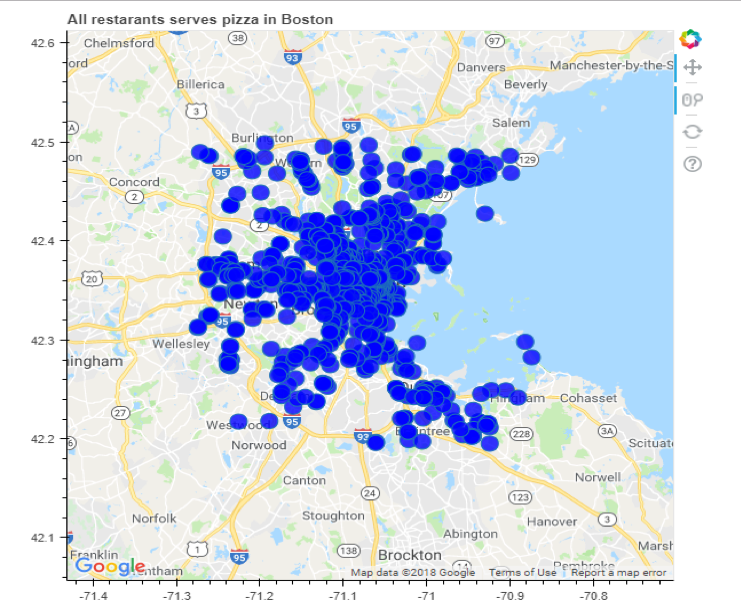
\includegraphics[width=0.8\textwidth]{Picture1.png}
\caption{\label{fig:data}All restaurants in Boston serves pizza on map }
\end{figure}

We set the cluster size to be 5, which is in accordance to the size of category of ratings (shown as stars) in Yelp dataset. The mean rating score of each cluster is calculated and sorted. Labels of number 1 to 5 are then attached the clusters according to their mean rating ranks in all mean ratings of those clusters. We can receive a Silhouette Coefficient of 0.423 with K-Means clustering, and a slightly larger 0.424 with GMM clustering, which means that both methods almost equal effect of separating these location data into different clusters.

As shown in the figure below, the K-Means clustering result of the locations of the restaurants are plotted out with the attached labels of ratings. We will suggest a user to go to the area colored yellow or green to find best and relatively cheap pizza restaurants in Boston.[2] 
\begin{figure}[htbp]
\centering
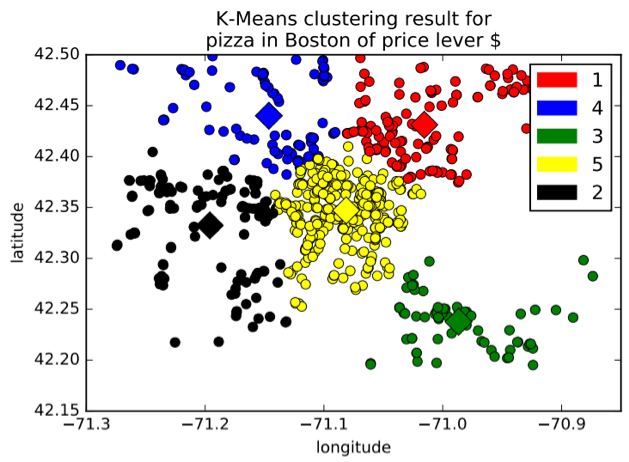
\includegraphics[width=0.8\textwidth]{Picture2.png}
\caption{\label{fig:data}K-Means clustering result for "pizza in Boston" of the required price level. Tag "5" stands for the best-rating restaurants and tag 1 stands for the worst ones, respectively }
\end{figure}


Additionally, using the same methods, we can explore if there is a part in Boston that has a particular price attributes. The clustering size set to be 4, which is in accordance with the price attributes in Yelp from \$ to \$\$\$\$. The K-Means clustering results in a silhouette score of 0.429 and GMM give a 0.471, which is better. Therefore GMM is adopted. As is shown in the figure below, we have the classification of 4 price range 1 to 4 and 4 indicates the most expensive restaurants that offers pizza in Boston. This is in accordance with the heat map of sale price of real estate in Boston.
\begin{figure}[htbp]
\centering
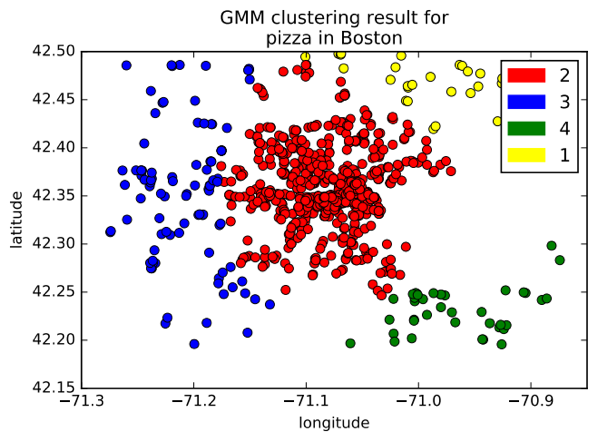
\includegraphics[width=0.8\textwidth]{Picture3.png}
\caption{\label{fig:data}GMM clustering result for "pizza in Boston". Tag "4" stands for the most expensive ones and tag "1" stands for the cheapest ones}
\end{figure}


\begin{figure}[htbp]
\centering
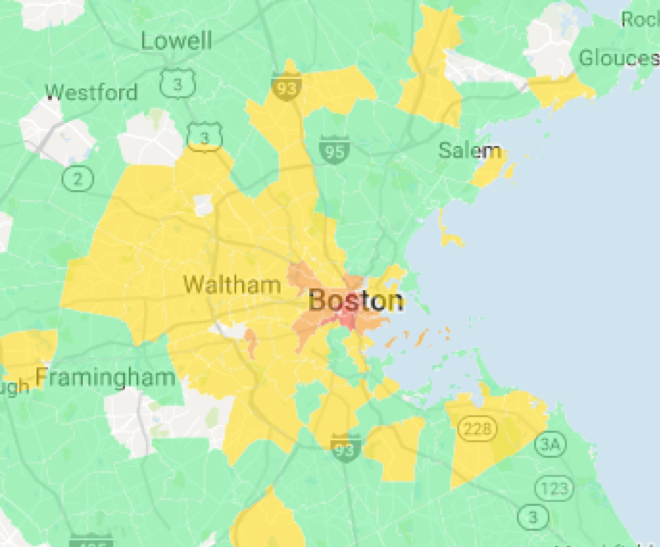
\includegraphics[width=0.6\textwidth]{Picture4.png}
\caption{\label{fig:data}Heat map of real estate sell price in Boston from trulia.com. }
\end{figure}
\
\\
\\
\subsection{NLP tasks by using TextBlob}
In this project, we'll use a Python library called TextBlob to perform simple natural language processing tasks. "Natural Language Processing" is a field at the intersection of computer science, linguistics and artificial intelligence which aims to make the underlying structure of language available to computer programs for analysis and manipulation. With respect to language processing, tokenization, filtering, lemmatization, and stemming were all used for preprocessing the reviews. 
Next, we extracted the top 50 keywords from positive and negative reviews. Again taking a sample dataset of all restaurants in Boston that have more than 200 reviews. Data processing techniques such as tokenizing, filtering, stemming and filtering the key words from those reviews were performed. We then calculated 50 most frequent keywords from the negative and positive reviews separately. Negative and positive reviews were distinguished using the polarity obtained in the previous step. The results are very promising. One important thing to notice is that "good" and "great" appeared in negative reviews too in a sense that customers are complaining how the food isn't that good/great. The high frequencies of words in positive reviews when compared to negative reviews is because of more number of positive reviews in the corpus. 


\subsection{Sentiment analysis by using Google Cloud Natural Language API}
To tell if a customer has positive or negative feedback about a restaurant, sentimental analysis was performed in order to see if there is an interesting difference between reviews and ratings although a review is associated with a rating. 
Google Cloud Natural Language API, a powerful text analysis tool, to inspect the emotional opinion of customers in reviews. The API attempts to determine the overall polarity of the text and is represented by numerical score and magnitude values. The score ranges between -1 and 1, and the magnitude corresponds to overall emotional leaning of the text. Scores greater than 0.25 is positive, and scores less than -0.25 is negative; anything in between is a neutral review. Magnitude determines the overall strength of emotion in the text. Unlike the score, magnitude is not normalized. 
In this project, we are more interested in highly positive reviews and highly negative reviews so that we can have a clear understanding of latent topics. We only considered the reviews whose magnitude is greater than 3 for our analysis. Below is a plot of sentiment distribution of reviews for different restaurants in Boston. 

\begin{figure}[htbp]
\centering
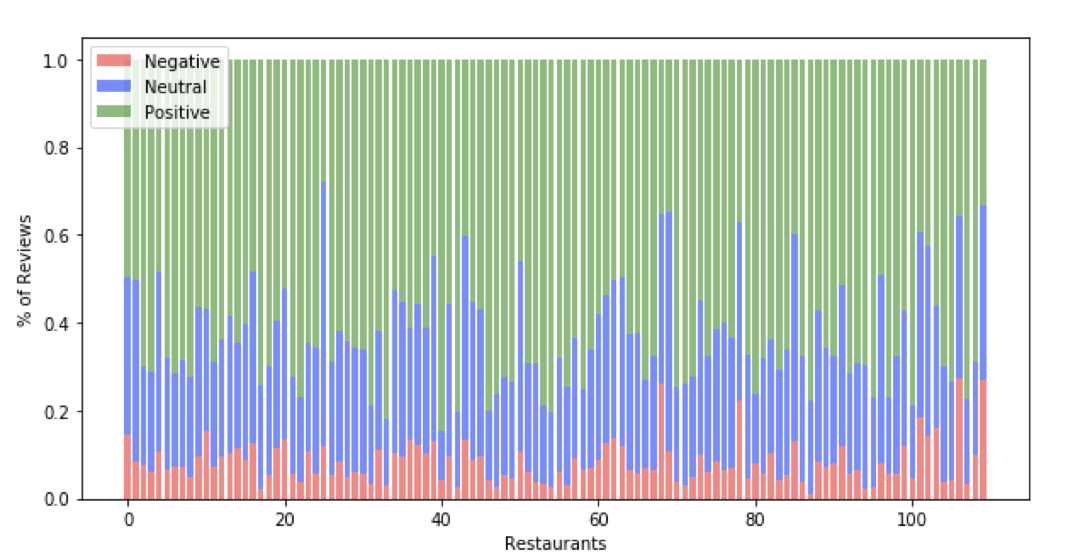
\includegraphics[width=1\textwidth]{Picture5.png}
\caption{\label{fig:data}Sentiment Analysis Result. }
\end{figure}

\subsection{LDA (Latent Dirichlet Allocation)}
In natural language processing, latent Dirichlet allocation (LDA) is a generative statistical model that allows sets of observations to be explained by unobserved groups that explain why some parts of the data are similar. LDA is an example of a topic model and was first presented as a graphical model for topic discovery by David Blei, Andrew Ng, and Michael I. Jordan in 2003.[3] 

In LDA, each document may be viewed as a mixture of various topics where each document is considered to have a set of topics that are assigned to it via LDA. This is identical to probabilistic latent semantic analysis (pLSA), except that in LDA the topic distribution is assumed to have a sparse Dirichlet prior. The sparse Dirichlet priors encode the intuition that documents cover only a small set of topics and that topics use only a small set of words frequently. 


\subsection{Gensim}
Gensim is a robust open-source vector space modeling and topic modeling toolkit implemented in Python. Gensim includes implementations of tf-idf, random projections, word2vec and document2vec algorithms, hierarchical Dirichlet processes (HDP), latent semantic analysis (LSA, LSI, SVD) and latent Dirichlet allocation (LDA), including distributed parallel versions.[4]



Our project is focused on the Yelp database. We collected 500?000 reviews within Boston as input. The output of LDA function is the topics with their related key words. To process the reviews (positive and negative), we break the text file into single words firstly, then we use LDA tools provided by python to mining topics and related key words in those reviews. To implement LDA more efficiently, we import Gensim.


\subsection{WordClouds}
After the file was processed, we use Word Cloud to reveal the words with high frequency. We generated some images. Again, reviews count less than 20 are filtered out and only terms that have occurred more than 10 times in the dataset will be thrown into the final model.
 
The words that occur with a higher frequency will be shown in larger front size. Figure 6 and 7 represent the positive results we have from part of the reviews. Data represented in figure 6 is from all the reviews we could extracted from Yelp and in figure 7, the words are extracted from the reviews about out topic 'pizza in Boston'. In figure 6, among the words with relative large front, we can notice words like 'place', 'people', 'chicken', 'price', 'sauce', and 'time' that is possibly worthwhile for the business owners to pay more attention to. In Figure 7, we can see that apart from the words mentioned above, words including 'delivery', 'quick', 'delicious', 'spot', 'staff', 'slice', 'service' and 'cheese' that might be crucial for a customer?s experience in a pizza restaurant. These words would provide some feedback to business owners.

\begin{figure}[htbp]
\centering
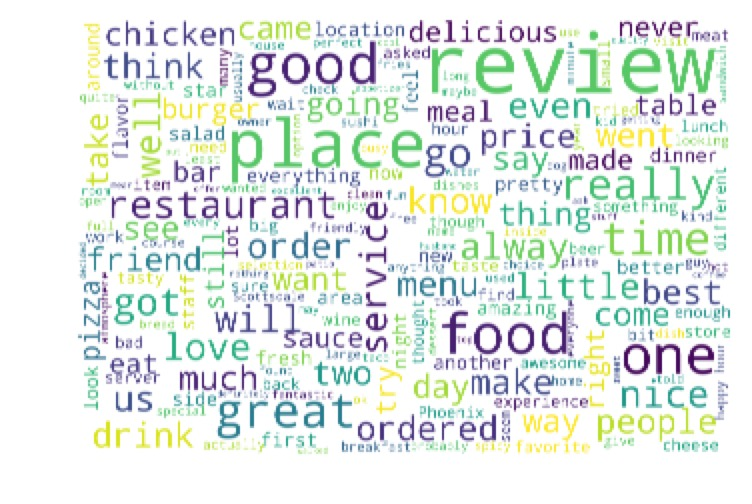
\includegraphics[width=1\textwidth]{Picture6.jpeg}
\caption{\label{fig:data}positive result via WordClouds 1. }
\end{figure}

\begin{figure}[htbp]
\centering
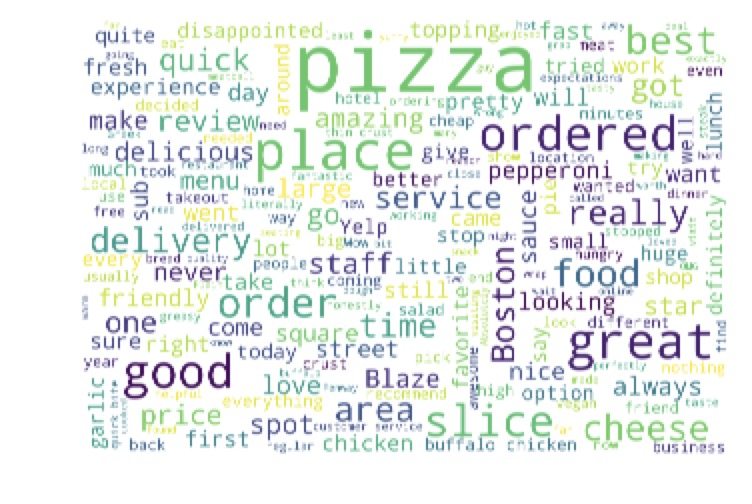
\includegraphics[width=1\textwidth]{Picture7.jpeg}
\caption{\label{fig:data} positive result via WordClouds 2. }
\end{figure}
\
\\
\\
\subsection{PyLDAVis}
PyLDAVis is a python library for interactive topic model visualization. It is designed to help users interpret the topics in a topic model that has been fit to a corpus of text data. The package extracts information from a fitted LDA topic model to inform an interactive web-based visualization. 
The left of Figure 2 is topics derived from the corpus. We derived 20 topics all together, based on the review database. The coordinate display their relavence. The right part is top frequent words of the reviews (unrelated words like ?am??is??are? are filterd due to over high frequency). 
The Figure 3 is top 1 of the result. The length of the bar represent the membership of a term in a particular topics. Besides visualizing topic precalence, the left pane showe inter-topic differences. The distance between two topics measuring similarity between two porbabilistic distributions. When topic 1 is clicked, the right panel of the visualization depict a horizental barchart. The red part of the bar chart represent how much this word counts in the total sample.most of them count more than the half.

\begin{figure}[htbp]
\centering
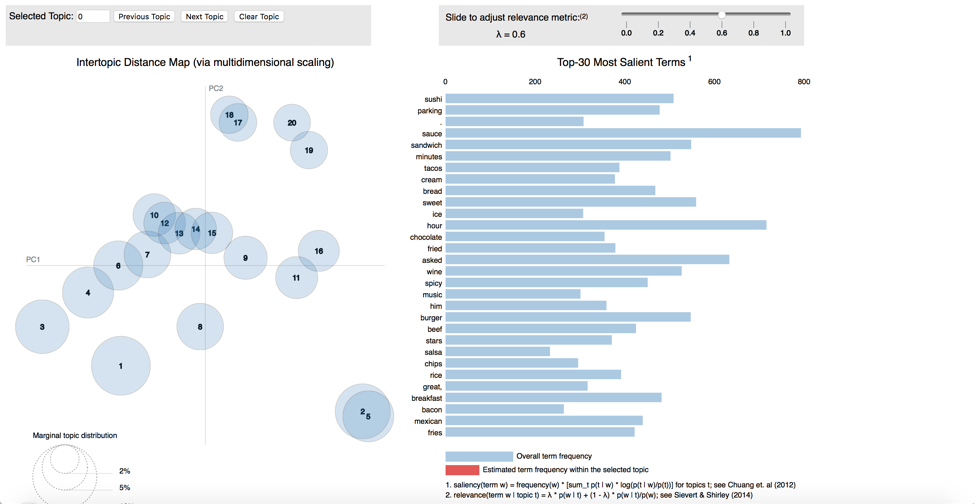
\includegraphics[width=1\textwidth]{Picture8.png}
\caption{\label{fig:data} LDA result via PyLDAVis. }
\end{figure}

\begin{figure}[htbp]
\centering
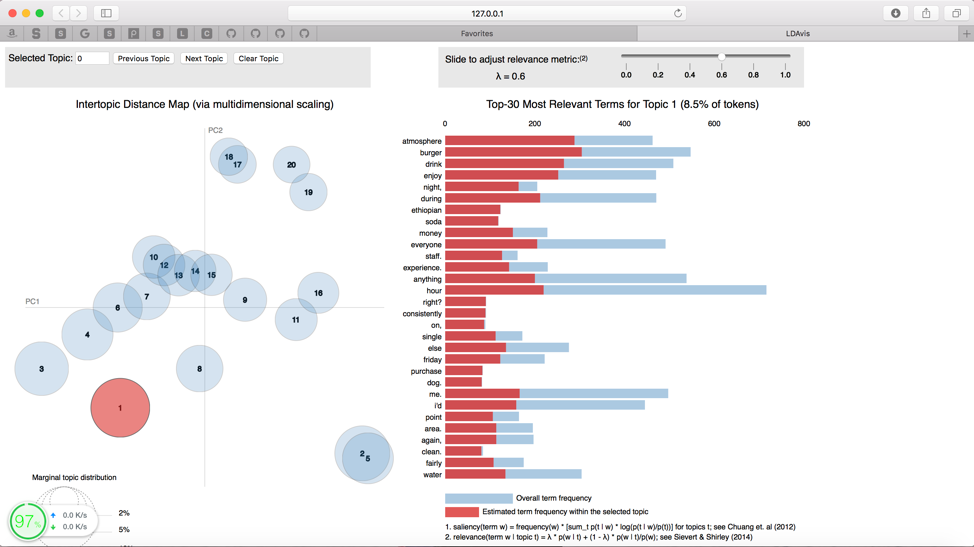
\includegraphics[width=1\textwidth]{Picture9.png}
\caption{\label{fig:data} topic 1 of LDA result. }
\end{figure}

The left of Figure 8 is topics derived from the corpus. The coordinate display their relavence. The right part is top frequent words of the reviews (unrelated words like 'am','is','are' are filterd due to over high frequency).
The Figure 9 is top 1 of the result. The red part of the bar chart represent how much this word counts in the total sample.most of them count more than the half
\
\\
\\
\section{Discuss}

The K-Means and GMM clustering methods using geographical location of restaurants cluster. Different labels of rating and pricing are attached to each cluster based on the mean rating and pricing of each cluster. However we still notice the problem that sometimes the average of one attribute in one clusters can be very close to the ones of others clusters. As we fail to upgrade out API to a VIP one, the dataset size we have is limited. If we could expand our dataset size, we might be able to see that the gap between the means will expand. Also, more cities can be explored in the future so that we can make sure that if there is a relationship between the location and rating, or location and price for a restaurants.

By doing sentiment analysis, we can see how much positive or negative reviews have occurred amongst customers. By combining the quantitative and the qualitative measurements, we can have a better measurement for marketing campaign. The information we get from sentiment analysis provides us with means to optimize the marketing strategy.

By clustering the restaurants within a specific area, we can find the distribution of restaurants. The result can give people useful information about where to open a restaurant.
To process LDA analysis, we did sentimental analysis firstly. The data is divided into positive and negative.
LDA results produce more instructive information. First, we can find what aspects guests most care about, it will give restaurants a direction how to improve themselves. Different topic may have different strategies, the PyLDAVis images serve as a good source to improve multitype restaurants.

\
\\
\\
\\
\\
\\
\\
\\
\\
\\
\\
\\
\\
\\
\\
\\
\\
\\
\\
\\
\\



\begin{thebibliography}{9}
\bibitem{nano3}
 https://www.yelp.com/about
 \bibitem{nano3}
 https://www.trulia.com/homeprices/Massachusetts
  \bibitem{nano3}
 Blei, David M.; Ng, Andrew Y.; Jordan, Michael I (January 2003). Lafferty, John, ed. "Latent Dirichlet Allocation". Journal of Machine Learning Research. 3 (4,5): pp. 9931022. doi:10.1162/jmlr.2003.3.4 5.993
 \bibitem{nano3}
Petr Sojka (2010). Software framework for topic modelling with large corpora. Proc. LREC Workshop on New Challenges for NLP Frameworks
\end{thebibliography}

\end{document}